\section{Platforms and Models}
\subsection{JuPedSim and Social Force Model}
JuPedSim \cite{chraibiJuPedSim2025} is an open-source software framework for pedestrian dynamics and personnel evacuation simulation, aiming to study the movement and evacuation behaviors of people in the built environment through computer simulation. This tool takes "self-driven multi-agent system" as its core concept, modeling each pedestrian as an independent agent. The agents follow a set of rules in a given scene to determine their own movement path, speed and interaction behavior, thereby presenting phenomena such as flow, congestion, queuing and path selection at the group level at the macro level. 

JuPedSim is assembled with pedestrian dynamics models such as the classic Social Force Model. The model defines three forces that influence pedestrian movement: the driving force, the repulsive force between pedestrians, and the repulsive force from obstacles. The driving force represents the agent's desire to reach a target position at a certain speed, while the repulsive force is caused by the interaction between the individuals and causes them to avoid each other in order to avoid collisions.The obstacle force acts in a similar way to the repulsive force to avoid collisions with obstacles.

The fundamental principle can be expressed by the following equation:
\begin{equation}
    m_i\underbrace{\frac{d\boldsymbol{v}_i}{dt}}_{\text{Acceleration}} = \underbrace{m_i \frac{\boldsymbol{v}_i^0(t)\boldsymbol{e}_i^0(t) - \boldsymbol{v}_i(t)}{\tau_i}}_{\text{Driving Force}} + \underbrace{\sum_{j(\neq i)} f_{ij} + \sum_W f_{iW}}_{\text{Interaction Forces}}
\end{equation}

Where \(m_i\) is the mass of pedestrian \(i\), \(\boldsymbol{v}_i(t)\) is the current velocity, \(\boldsymbol{v}_i^0(t)\) is the desired speed, \(\boldsymbol{e}_i^0(t)\) is the desired direction, and \(\tau_i\) is the relaxation time. The terms \(f_{ij}\) and \(f_{iW}\) represent the repulsive forces from other pedestrians and obstacles, respectively.

Specifically, the repulsive force between pedestrians \(f_{ij}\) can be expressed as:
\begin{equation}
    f_{ij}^{repulsive} = \underbrace{A_i \exp\left(\frac{r_{ij} - d_{ij}}{B_i}\right) \mathbf{n}_{ij} + k g(r_{ij} - d_{ij}) \mathbf{n}_{ij}}_{\text{Pushing}} + \underbrace{\kappa g(r_{ij} - d_{ij}) \Delta v_{ji}^t \mathbf{t}_{ij}}_{\text{Friction}}
\end{equation}

Where \(A_i\) and \(B_i\) are constants representing the strength and range of the repulsive force, \(r_{ij}\) is the sum of the radii of pedestrians \(i\) and \(j\), \(d_{ij}\) is the distance between them, \(\mathbf{n}_{ij}\) is the unit vector pointing from pedestrian \(j\) to \(i\), \(\mathbf{t}_{ij}\) is the tangential unit vector, \(k\) and \(\kappa\) are constants related to body compression and friction, and \(g(x)\) is a function that equals \(x\) if \(x > 0\) and 0 otherwise.

The obstacle force from  \(f_{iW}\) is similarly defined as:
\begin{equation}
    f_{iW}^{obstacle} = \underbrace{A_i \exp\left(\frac{r_i - d_{iW}}{B_i}\right) \mathbf{n}_{iW} + k g(r_i - d_{iW}) \mathbf{n}_{iW}}_{\text{Pushing}} + \underbrace{\kappa g(r_i - d_{iW}) (\mathbf{v}_i \cdot \mathbf{t}_{iW}) \mathbf{t}_{iW}}_{\text{Friction}}
\end{equation}

Where \(r_i\) is the radius of pedestrian \(i\), \(d_{iW}\) is the distance to the obstacle, \(\mathbf{n}_{iW}\) and \(\mathbf{t}_{iW}\) are the normal and tangential unit vectors relative to the obstacle.

The velocity can be updated using the following equation:
\begin{equation}
    \boldsymbol{v}_{new} = \boldsymbol{v}_i(t) + \frac{d\boldsymbol{v}_i}{dt} \Delta t
\end{equation}

From the above equations, it can be seen that the velocity of each agents is influenced by its own driving force, as well as the pushing forces and fricional forces with other pedestrians and obstacles. 

\subsection{Rhino3D and Grasshopper}
Rhino3D \cite{RhinoRhinoceros3D} (also known as Rhino or Rhinoceros3D) is a 3D modeling software developed by Robert McNeel Associates, widely used in architecture, industrial design, and many other fields. Grasshopper is a visual programming language and environment integrated into Rhino, allowing users to create complex parametric models through a node-based interface.

The study's modeling and simulation workflow are conducted in Rhino 9 WIP, using Rhino as the geometry and initial agents placement environment \ref{fig:rhinoandgrasshopper}. Grasshopper serves as the parametric front-end to drive the simulations, passing geometric inputs (polylines, doors, corridors, etc.) as point lists to the agent-based simulation instance.

Grasshopper is extended via Python scripting to enable integration with JuPedSim \ref{fig:rhinoandgrasshopper}. An assembled Python 3.13 environment is used to write the scripts that map Rhino/Grasshopper geometry to JuPedSim input scenes and to extract trajectories and scene metadata from JuPedSim outputs for analysis. We didn't use Rhino before version 9 WIP because it is the first version that supports Python 3.13 (Rhino 8's Python is 3.9), which is required by JuPedSim.

\begin{figure}
    \centering
    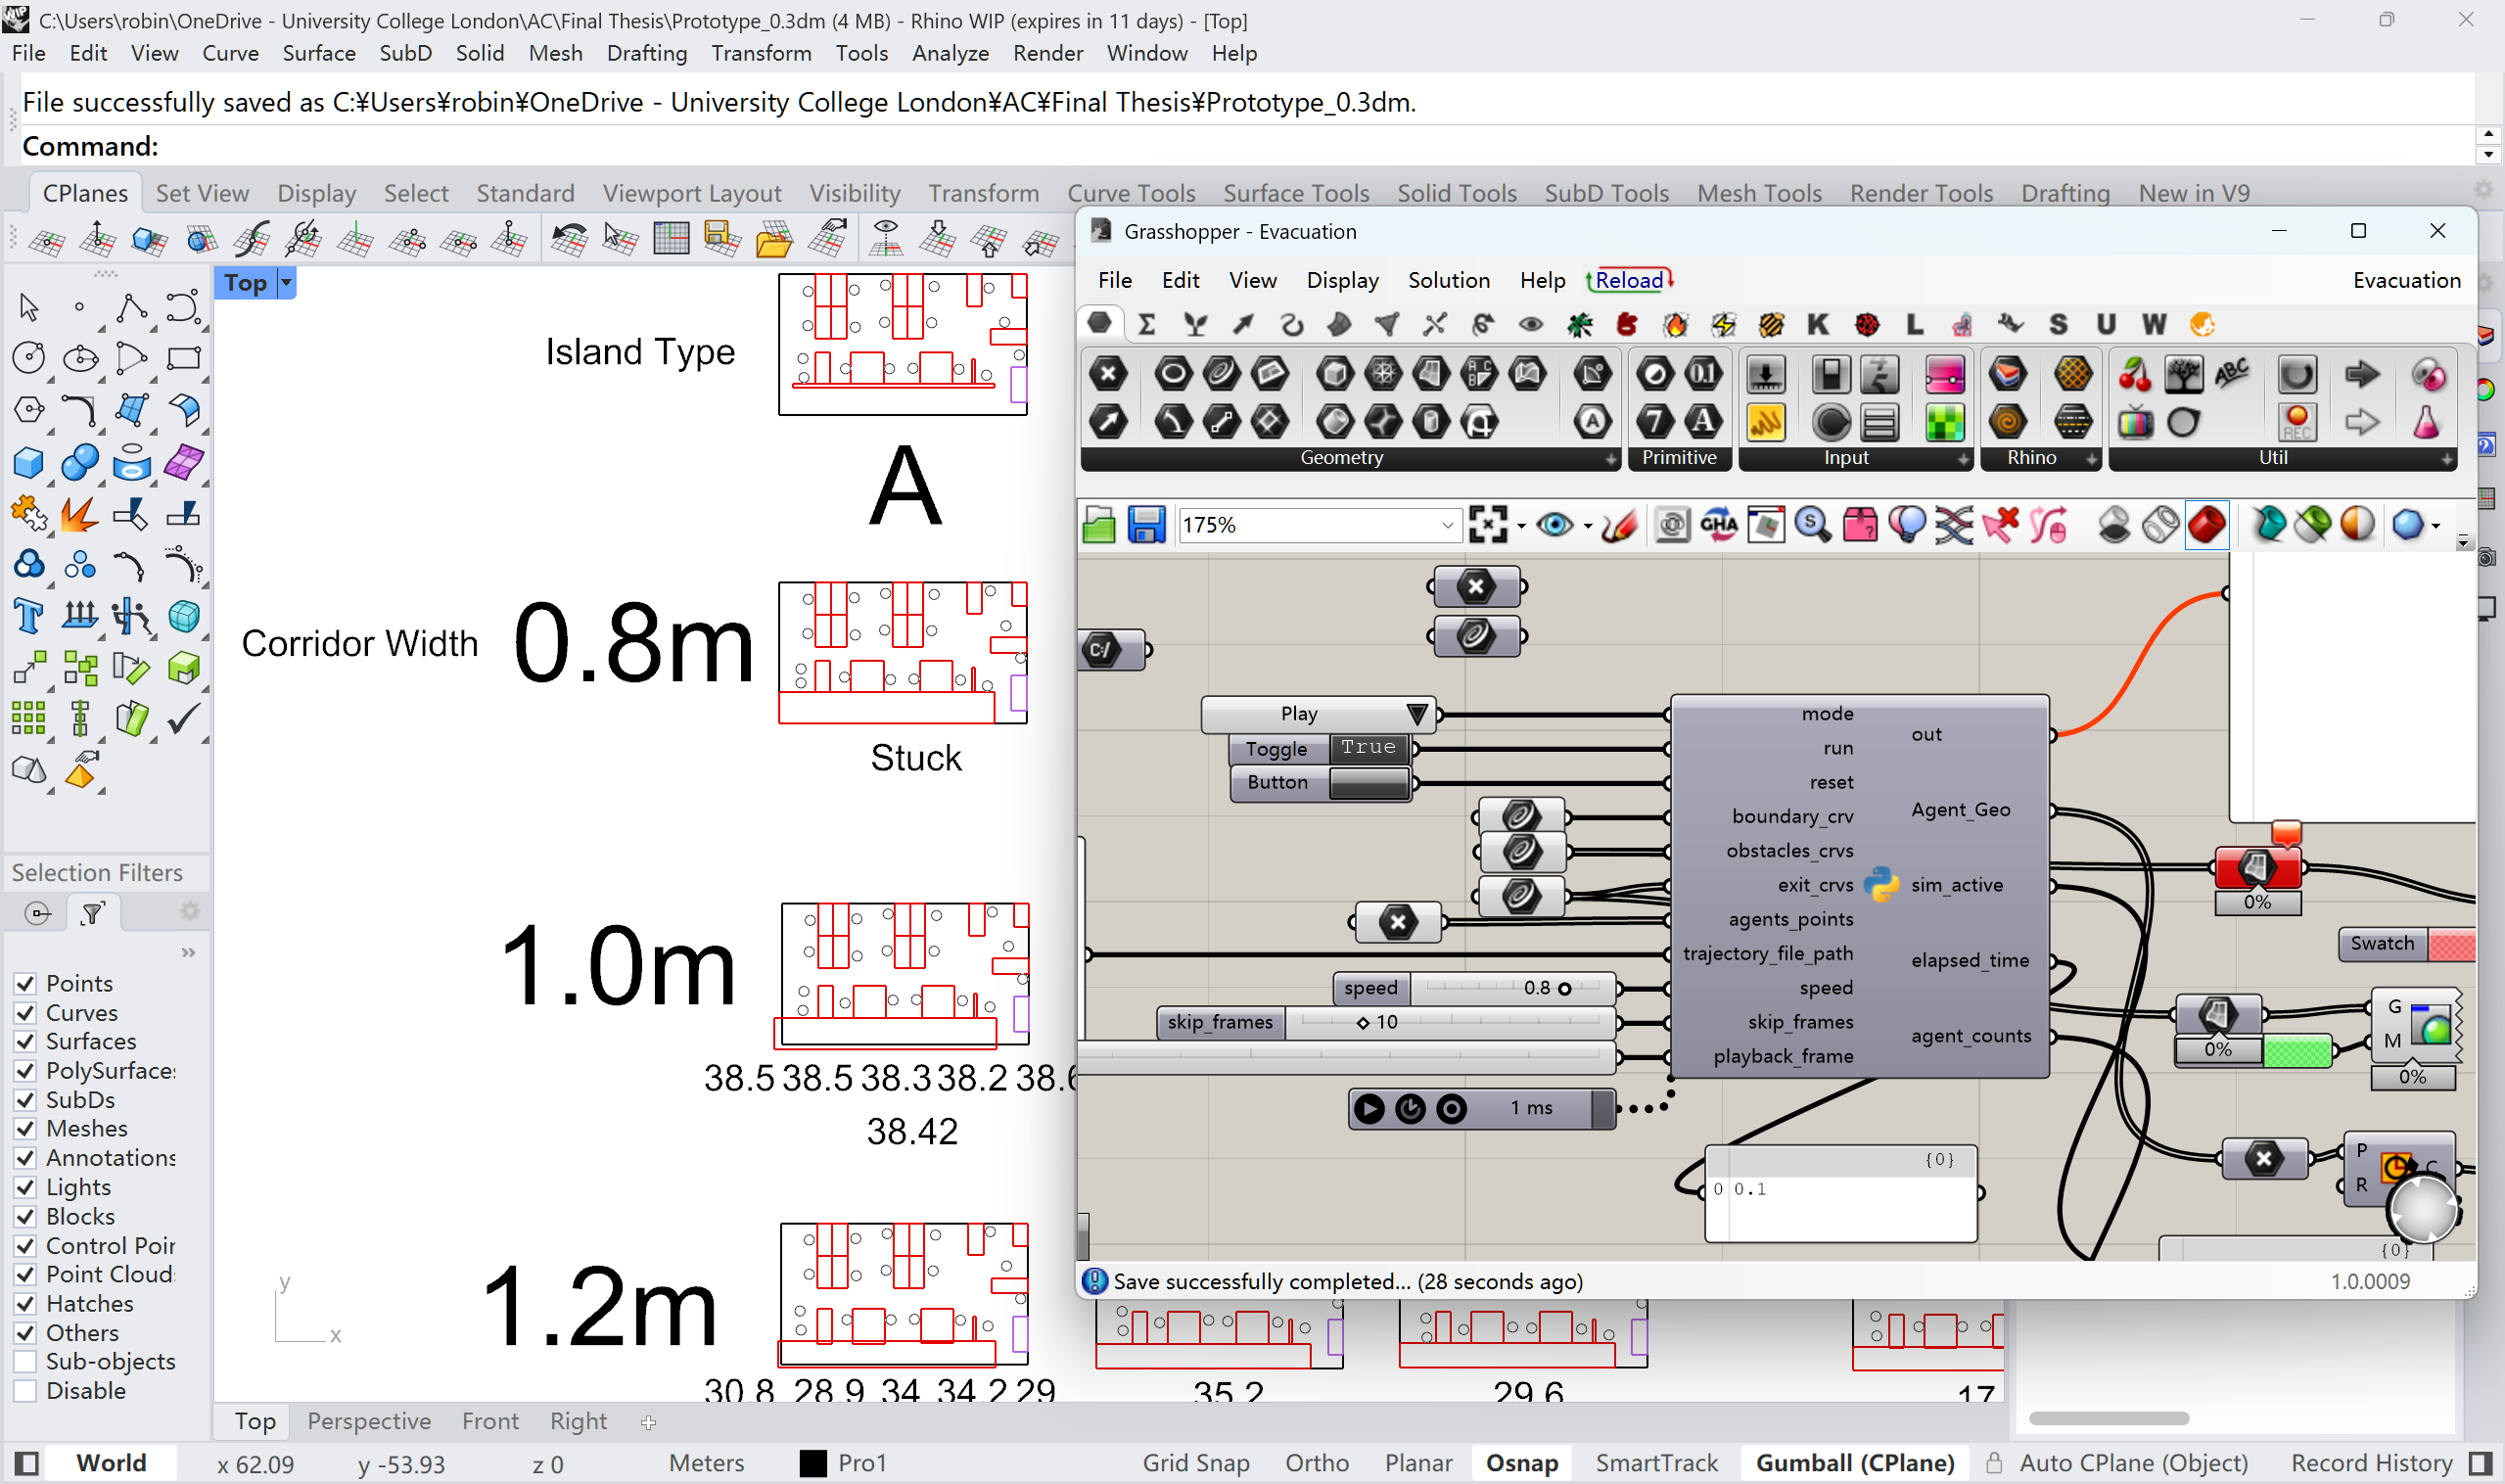
\includegraphics[width=\textwidth]{Rhino&Grasshopper.png}
    \caption{Rhino and Grasshopper}
    \label{fig:rhinoandgrasshopper}
\end{figure}

\section{System Integration}
\subsection{Objectives and Framework}
Standard JuPedSim uses the Shapely package for geometry input and visualization, which limits efficiency when generating multiple experimental prototypes and offers limited parametric control. This study based on Rhino3D's parametric modeling environment,using a Python script \ref{fig:pythonscript} to integrate geometric data and call JuPedSim's API to run the simulation, in order to conveniently generate prototypes and systematically control parameters during each experiment.

\subsection{Input and Output Description }
As the figure \ref{fig:pipeline} shows, Geometric inputs define the physical space through polyline(stored as point list) representations of the office layout, including office space boundaries that establish the walkable area, obstacle geometries that represent furniture or colunms, and exit locations. Additionally, the system requires agent positioning data provided as a point list that specifies the initial locations where pedestrians will be placed before the simulation. 

Each simulation run generates an individual SQLite file that stores all simulation results. The file stores trajectory data including frames, agent id, agent coordinates per frame, and orientation vectors per frame. The file also preserves simulation metadata and geometric data of the walkable area, allowing subsequent analysis and playback.'

\begin{figure}[h]
    \centering
    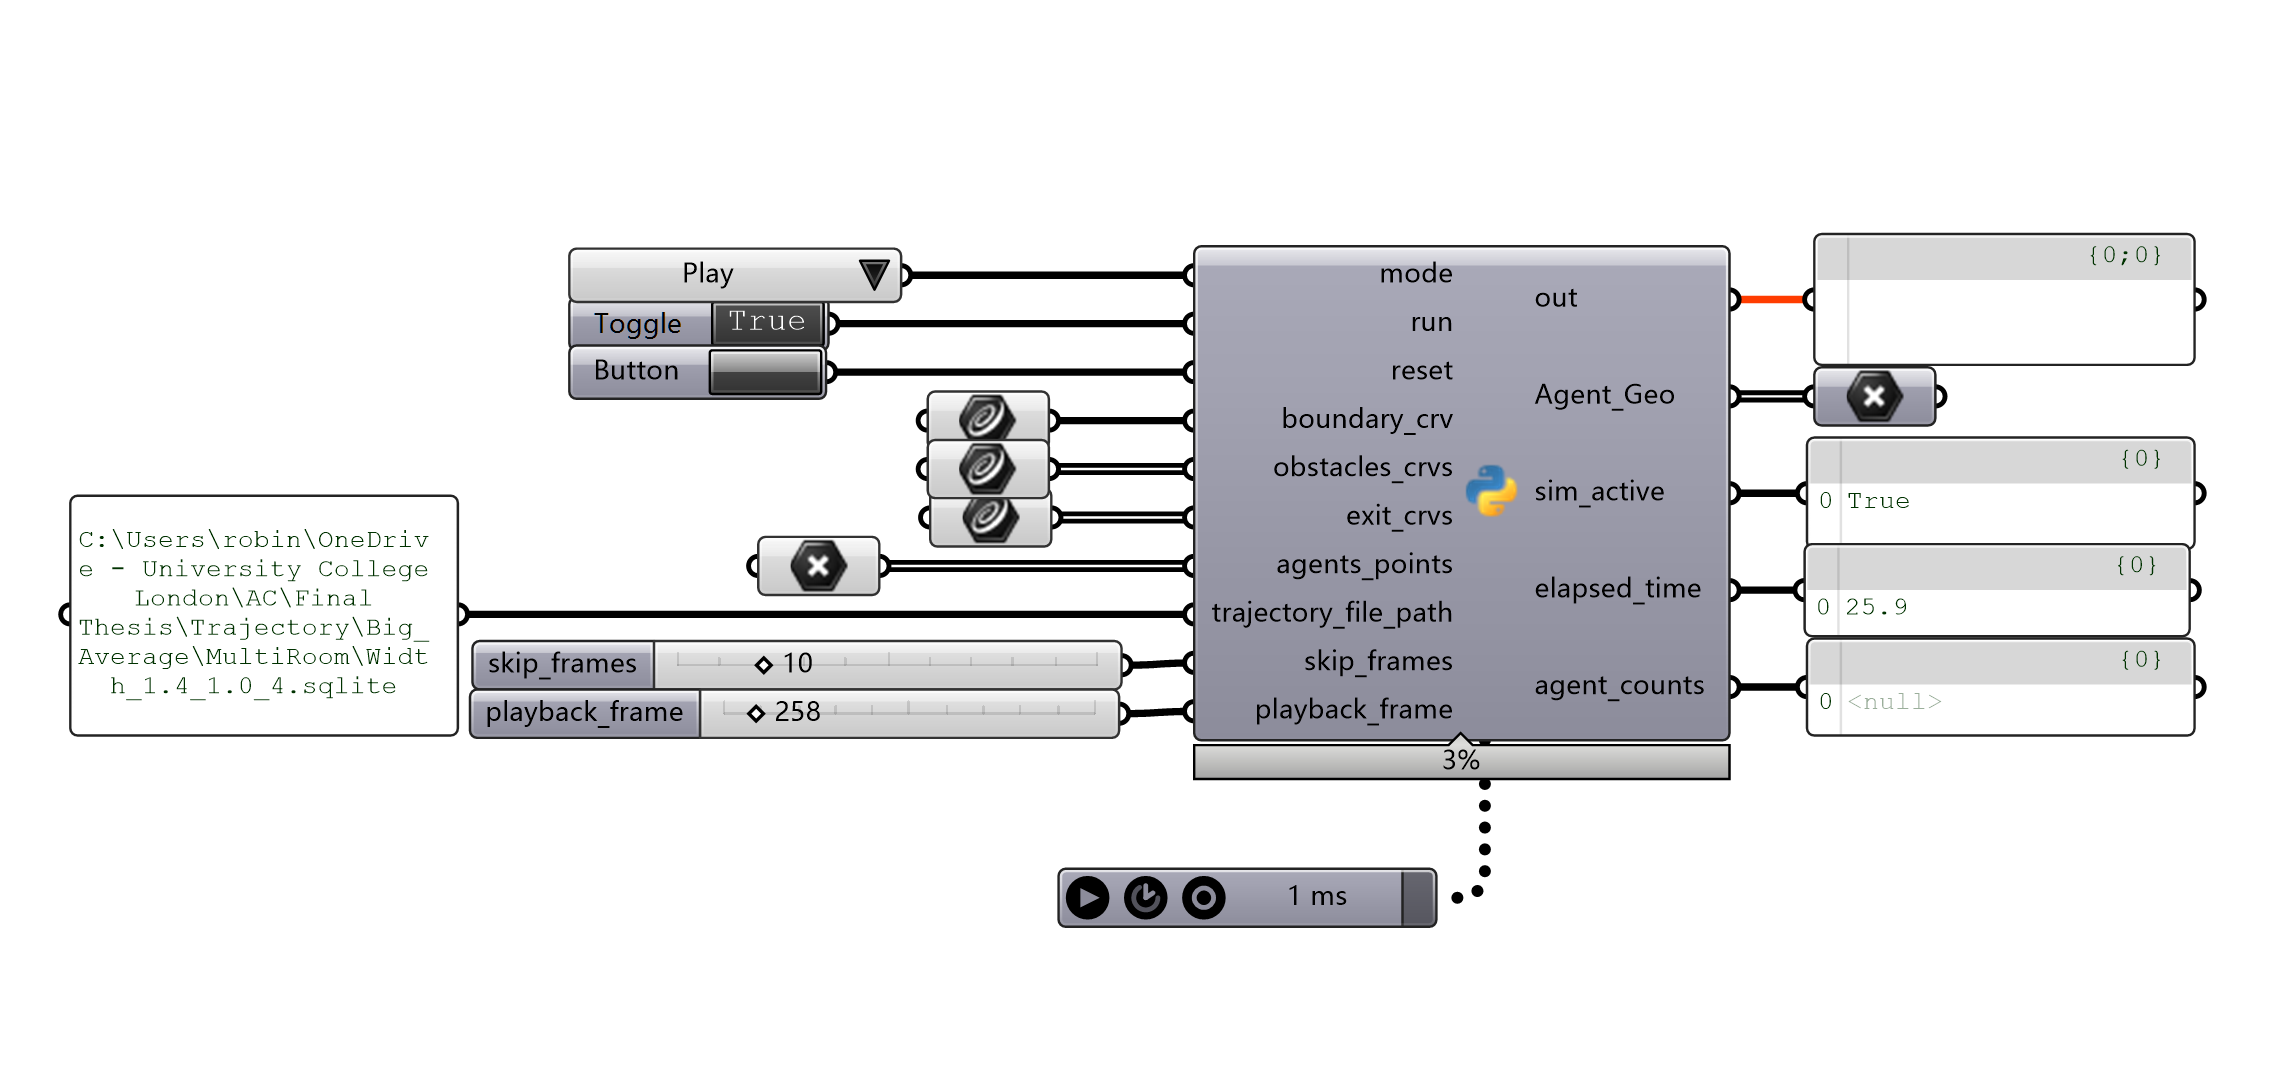
\includegraphics[width=\textwidth]{PythonScript.png}
    \caption{Python Script in Grasshopper for JuPedSim Integration}
    \label{fig:pythonscript}
\end{figure}

\begin{figure}[h]
    \centering
    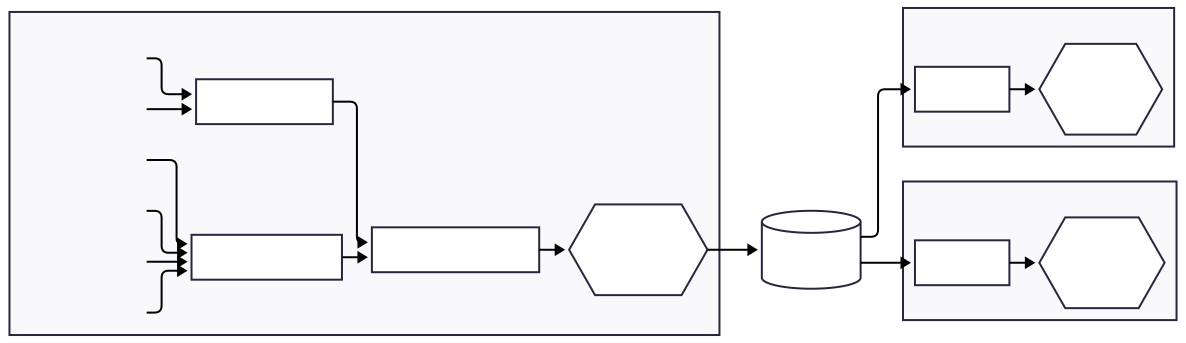
\includegraphics[width=\textwidth]{DataPipeline.svg}
    \caption{Data Pipeline}
    \label{fig:pipeline}
\end{figure}

\section{Experimental design}

\subsection{Prototype Scales}
Small prototype \ref{fig:small}: Focus on the preliminary effects of layout on evacuation paths and times, with rapid iteration through smaller geometric dimensions. To eliminate the influence of multiple corridors, we extended the bottom wall to the leftmost and bottommost sides, keeping only the Main corridor while controlling its width.
\begin{figure}[h]
    \centering
    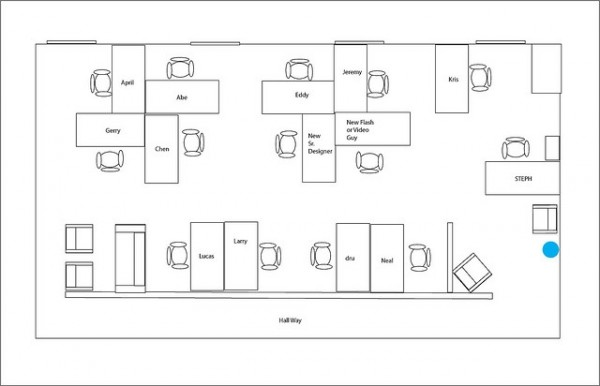
\includegraphics[width=\textwidth]{Small.jpg}
    \caption{Small Prototype}
    \label{fig:small}
\end{figure}
\\Big prototype \ref{fig:big}: Introduce higher-level issues such as door width coupling and multi-room nesting, testing the coupling effects at scales closer to actual office spaces.
\begin{figure}[h]
    \centering
    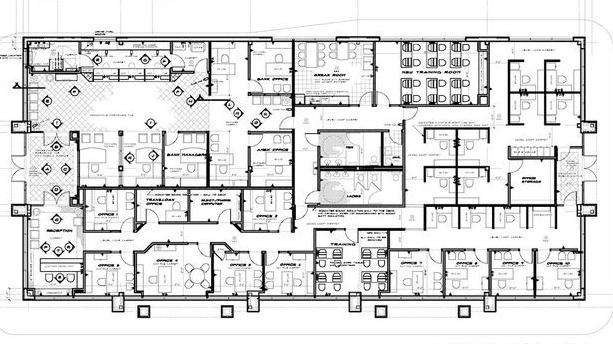
\includegraphics[width=\textwidth]{Big.jpg}
    \caption{Big Prototype}
    \label{fig:big}
\end{figure}

\subsection{Randomness and Replication}
Each parameter configuration is repeated 5 times, with initial positions randomly sampled from a Grasshopper point set to reduce the impact of randomness on the results.

\subsection{Small Prototype Variables}
Island Table Layout \ref{fig:abc}: Three variants A, B, and C represent the internal furniture configuration's representative parameters.
\begin{figure}[h]
    \centering
    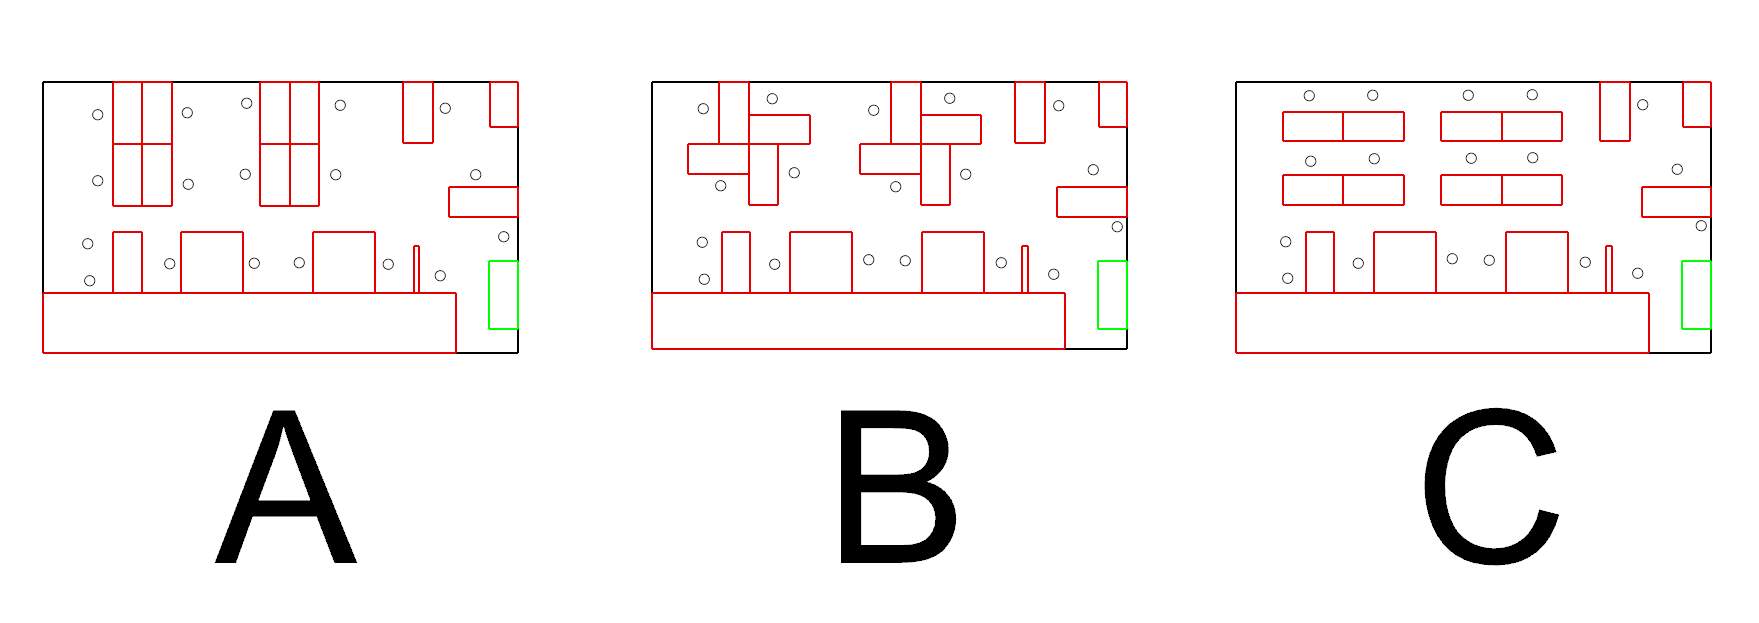
\includegraphics[width=\textwidth]{abc.png}
    \caption{Island Table Layout}
    \label{fig:abc}
\end{figure}

Corridor Width \ref{fig:corridorwidth}: 0.8 m,1.0m, 1.2 m, 1.4m, 1.6 m, 1.8m, 2.0 m, 2.2m, 2.4 m to explore the sensitivity of corridor width on path formation and congestion.
\begin{figure}[h]
    \centering
    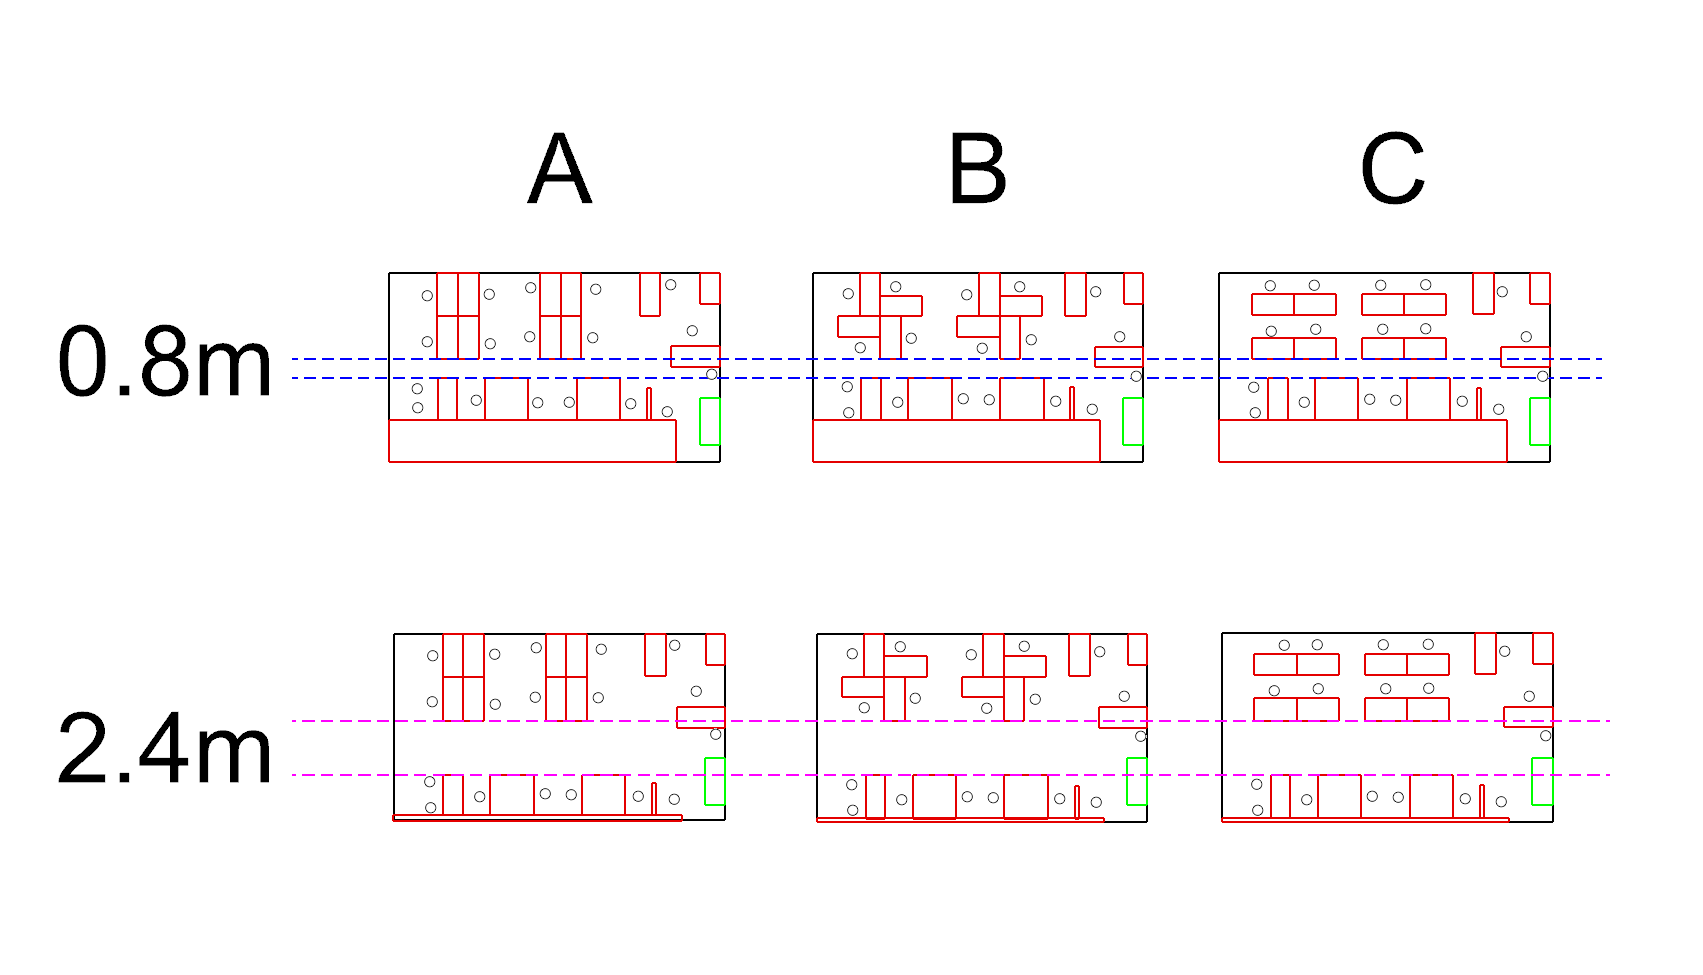
\includegraphics[width=\textwidth]{WidthCompare.png}
    \caption{Corridor Width}
    \label{fig:corridorwidth}
\end{figure}

Exit Configuration \ref{fig:ExitConfiguration}: Single exit and double exit, comparing the impact of different exit quantities on path formation and congestion.
\begin{figure}[h]
    \centering
    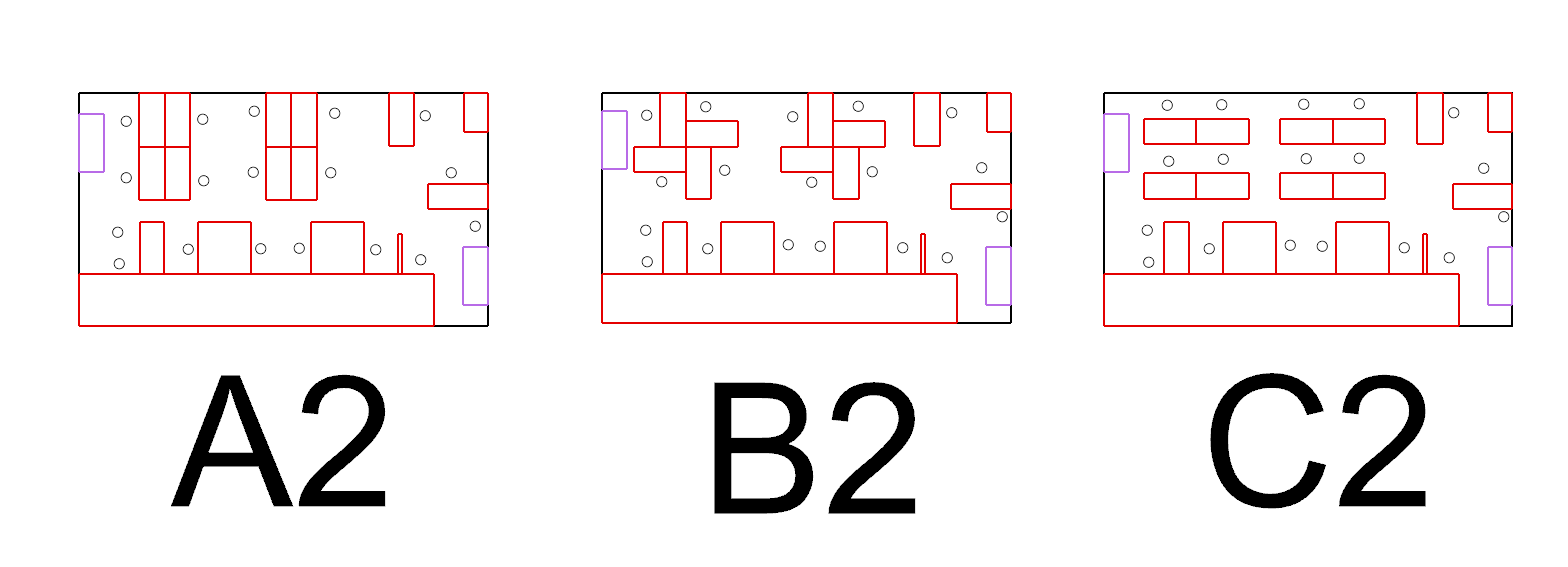
\includegraphics[width=\textwidth]{abc2.png}
    \caption{Exit Configuration}
    \label{fig:ExitConfiguration}
\end{figure}

\subsection{Big Prototype Variables}
We firstly conducted a primitive simulation on the original big prototype. And then we designed two main variable groups based on the primitive simulation results:
\\
Gate width before the exit(the bottleneck) \ref{fig:4ExitsGate}:
\(g\in[1.0,1.6]\text{m}\) is to assess sensitivity of early queuing, discharge rate, and lane merging.
\begin{figure}[h]
    \centering
    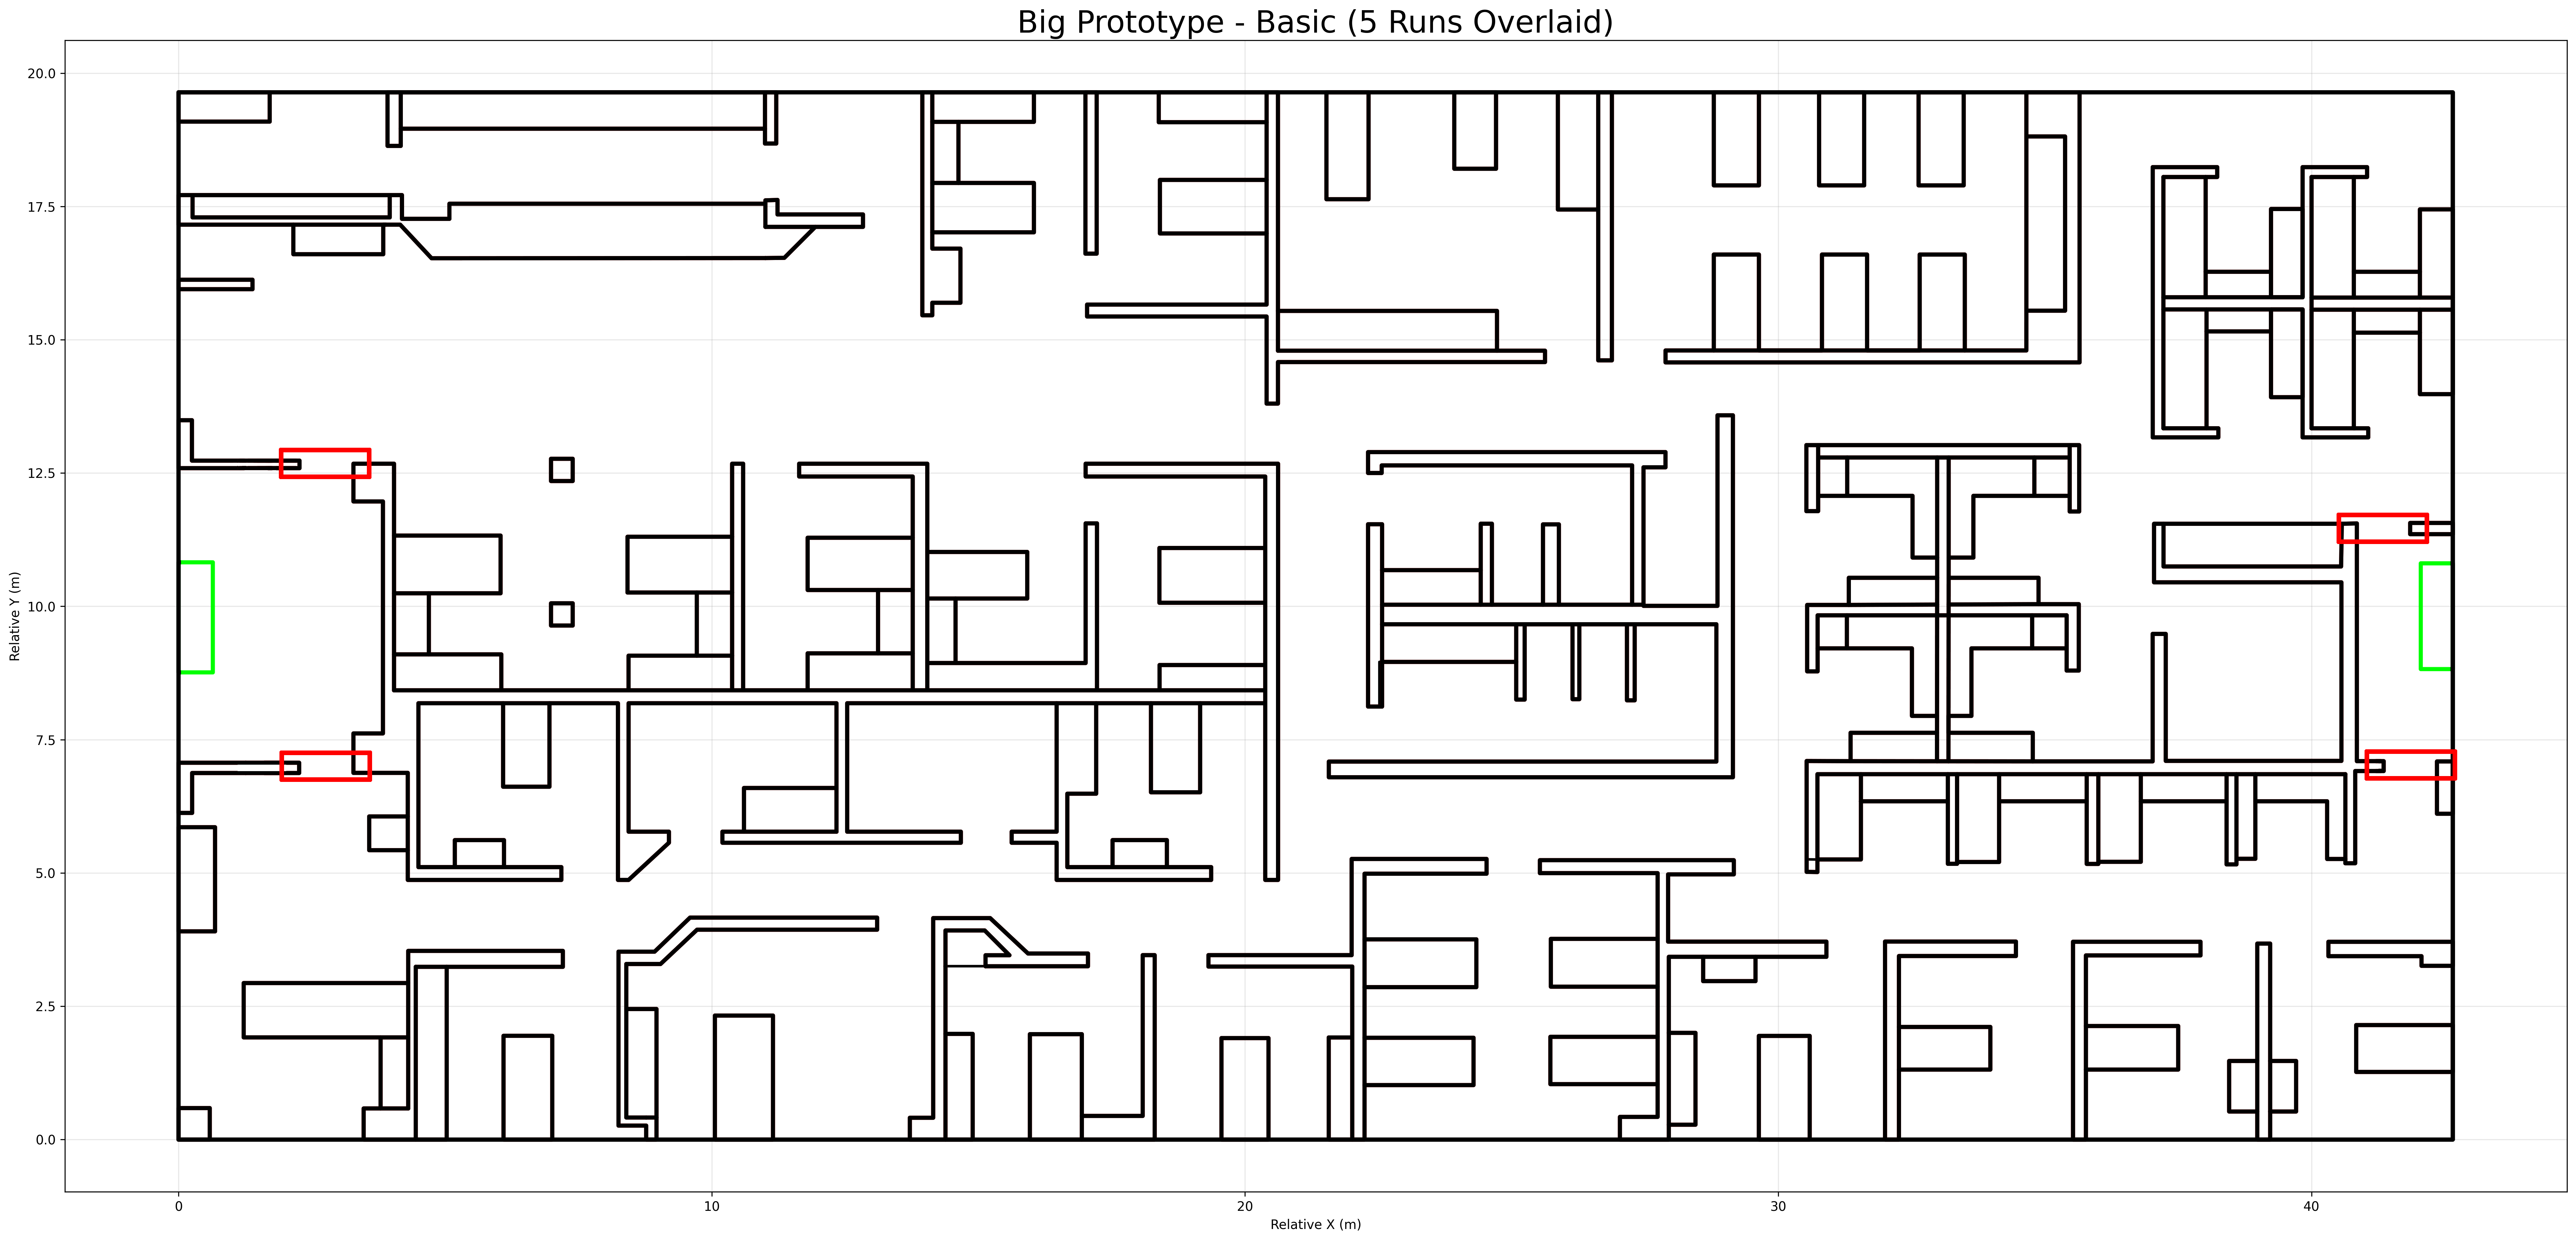
\includegraphics[width=\textwidth]
    {trajectory_overlay_layout_4ExitsGate.png}
    \caption{Change of the gates width before the exits}
    \label{fig:4ExitsGate}
\end{figure}
\\Room-Corridor Coupling: According to the primitive simulation \ref{fig:bigprimitive}, with red lines in the figure representing agent trajectories from all the five runs, the trajectories show convergence into three main corridor segments: corridor a (upper), corridor b (lower-left), and corridor c (lower-right). To quantify the combined effects of "room entrance(blue) and corridor gate(red) width" on the flow distribution and congestion of these main passages, we conducted a full factorial cross-experiment using room door width and corridor gate width entering a/b/c as core independent variables: room door width and gate width in range of {1.0, 1.2, 1.4, 1.6}m. For each combination, we evaluated its impact on early queuing, throughput capacity, and the merging and conflict patterns of the three corridors. 
\begin{figure}[h]
    \centering
    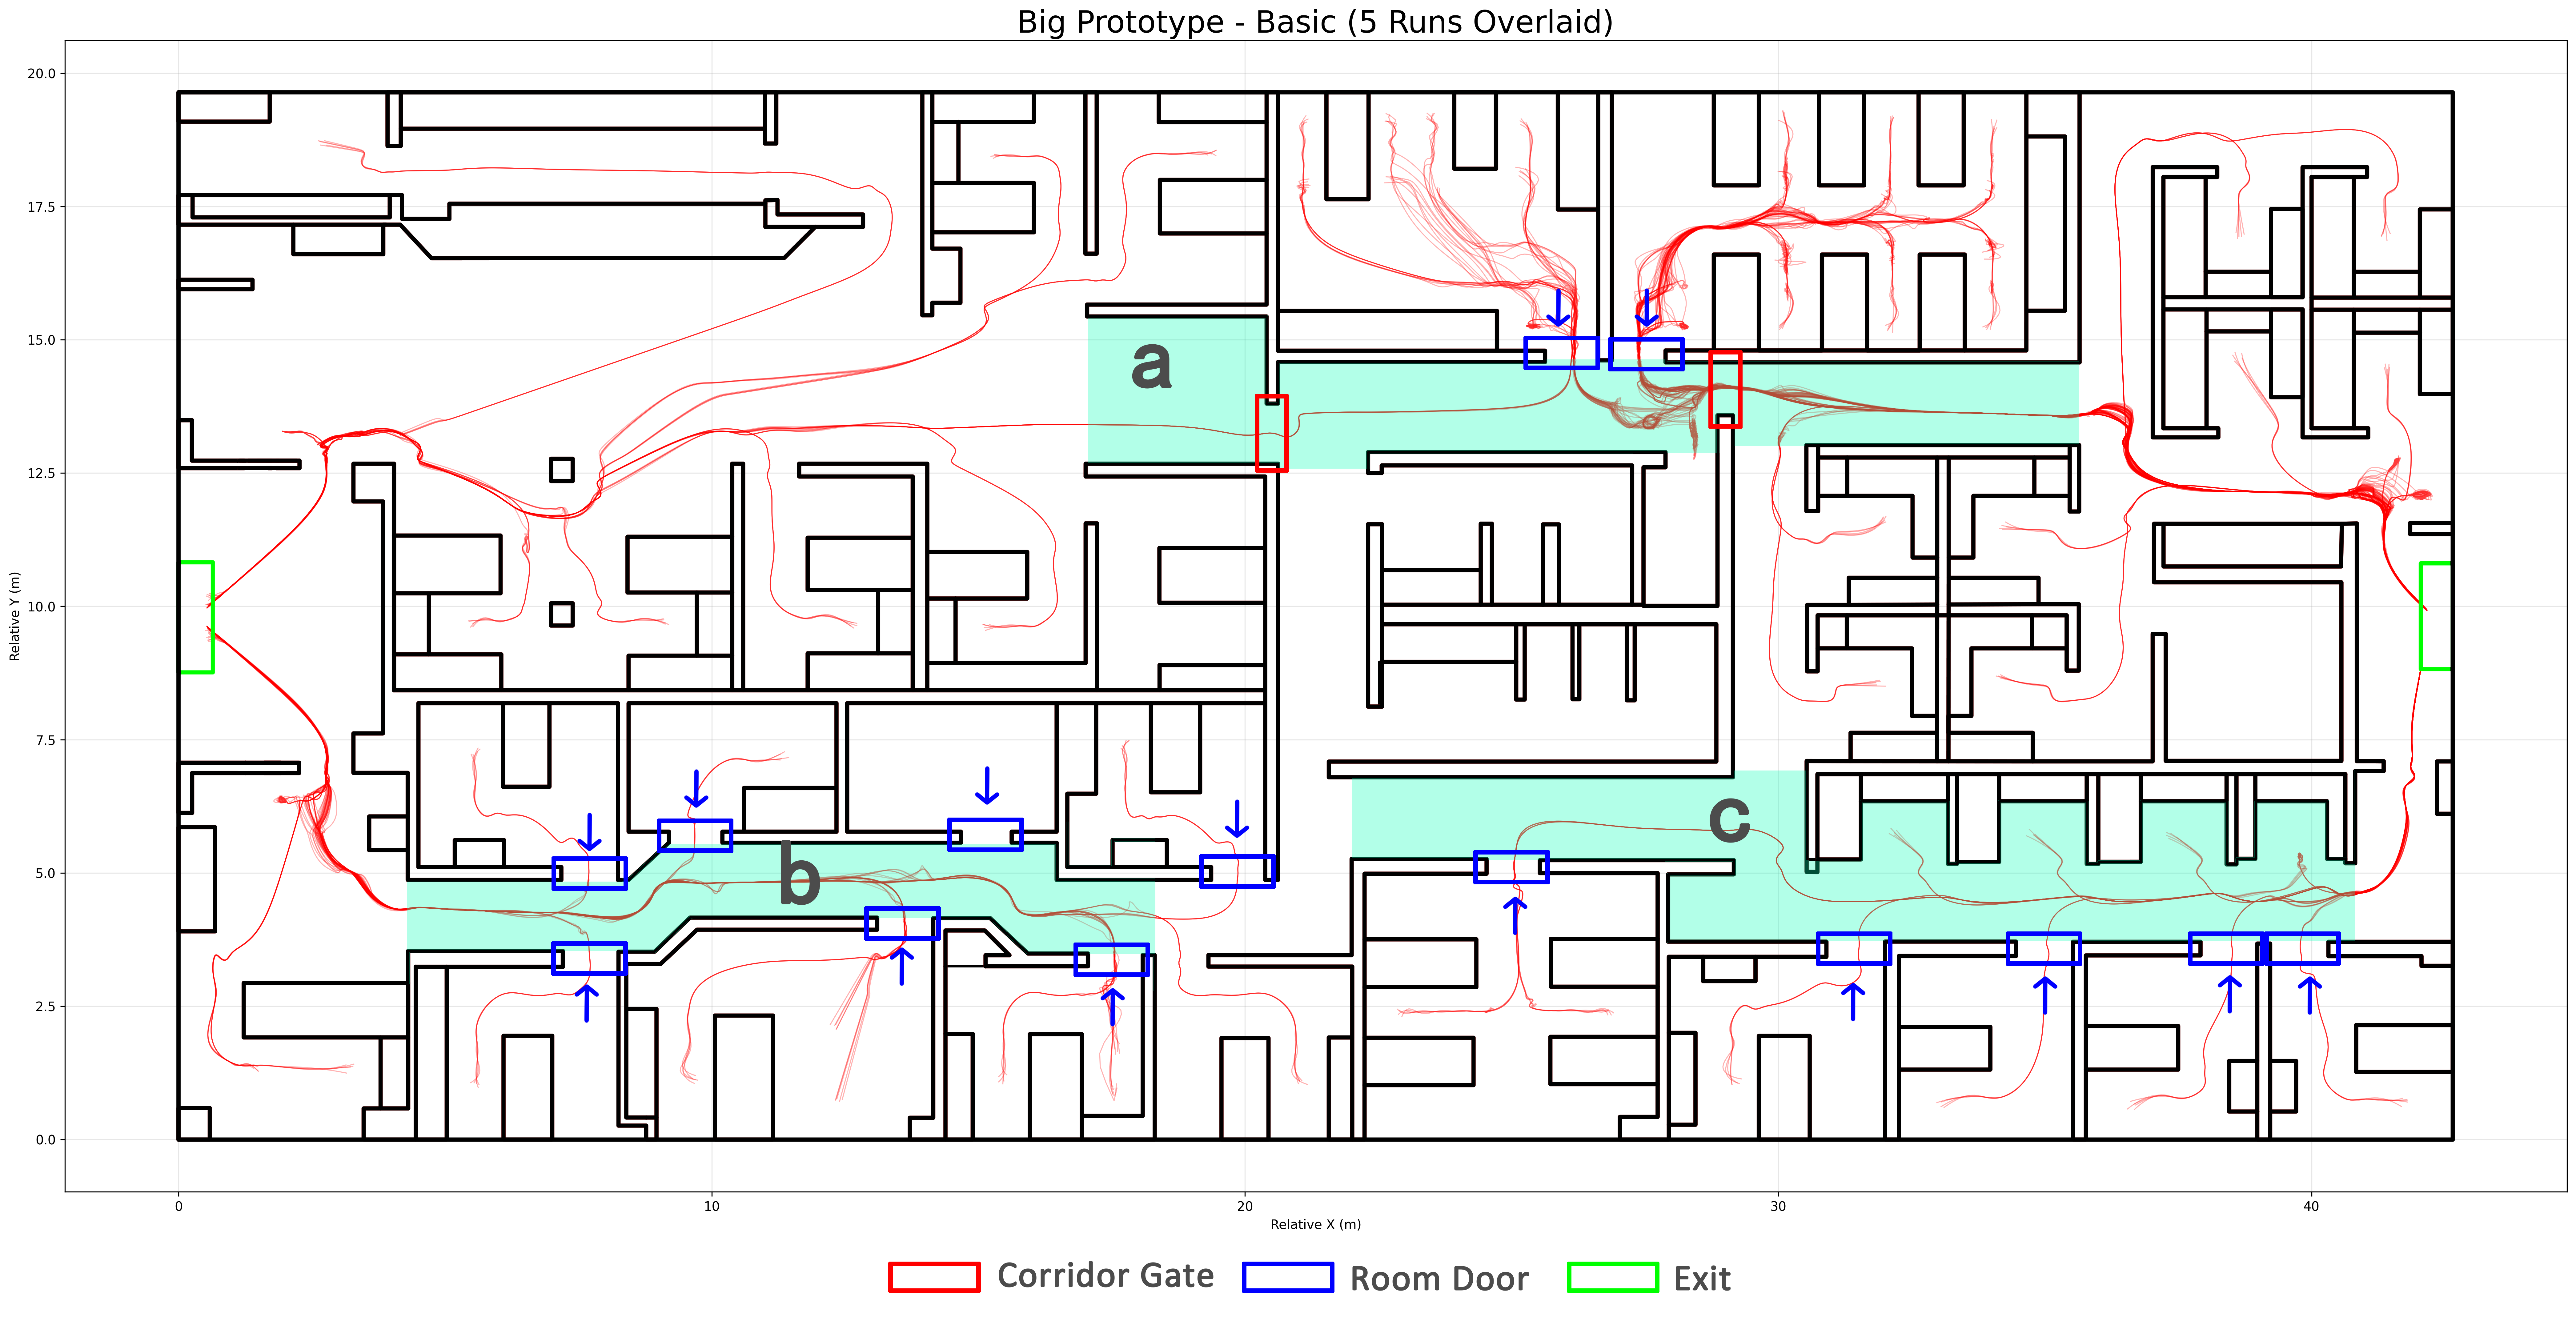
\includegraphics[width=\textwidth]{trajectory_overlay_layout_CorridorAnalysis_Basic.png}
    \caption{Trajectories on the original big prototype and main corridor segments}
    \label{fig:bigprimitive}
\end{figure}

\section{Agents and Model Settings}

This section focuses on clearly setting and recording the attributes of agents (pedestrians), the initial distribution, and the key parameters of the Social Force Model (SFM) within the JuPedSim framework, ensuring comparability and repeatability between different configurations.

\subsection{Agent Attributes and Initial Conditions}

Initial Agent Quantity and Distribution: The total number of agents is set in the Grasshopper/JuPedSim scene input based on the scale of the scenario, with the initial distribution (Grasshopper point set) controlling the initial quantity and spatial distribution.
\\Initial Position Mapping: The point set of Grasshopper is mapped to the initial coordinates of the agents, ensuring that the randomness of initial positions between different configurations is controllable and that repeated experiments can be replicated.
\\Goals and Behavioral Tendencies: Defaults are uniformly set, but in scenarios with multiple entrances, agents tend to choose the shortest path.

\subsection{Social Force Model Parameters}

Model Framework: The built-in Social Force Model of JuPedSim is used as the core microscopic simulation model.
\\Desired Speed: 0.8 m/s is set as the default value, with sensitivity analysis within a range (e.g., 0.6-1.0 m/s) conducted as needed.
\\Interaction Force Parameters: These include repulsive forces between agents, repulsive forces against obstacles, and response intensity to queuing and group aggregation. The initial settings adopt the official recommended values from JuPedSim.
\\Obstacle Handling and Boundary Conditions: The obstacle force scale is set to 1000 to balance the resistance to obstacles in complex scenarios, preventing excessive suppression of agent movement. Boundary conditions follow the wall and exit definitions in the geometric input of the scene.

\section{Data collection and Analysis}

\subsection{Data Output and Storage}
Each simulation produces an independent SQLite database file, recording agent trajectories, speeds, positions, and scene metadata for easy playback and offline analysis.
\subsection{Data Reading and Processing}
Use JupyterLab and Python to read SQLite files (sqlite3), organizing the data into an analyzable structure (DataFrame), and aggregating and statistics on time steps, agent attributes, congestion indicators, etc.

\subsection{Indicators}
\subsubsection{Primary Indicators}
Total Evacuation Time (TET): The overall comparison of evacuation performance under various configurations, which can be presented by evacuation time tables and line charts.
\\
Path Distribution Characteristics: Visualized through trajectory patterns in speed-trajectory diagrams.
\\
Congestion Hotspot Distribution (Hot Zones/Density): The location and extent of low-speed clustering and congestion areas in speed-trajectory diagrams, which equivalently display congestion hotspots and their migration patterns.
\\
\subsubsection{Secondary Indicators}
Path Formation Patterns: Identification of single-lane and double-lanes flow, lane convergence, bottleneck queuing patterns, and their locations based on the trajectory morphology analysis.
\\
Repeated Interval Fluctuation (Robustness): Line overlap/error band performance across multiple runs under identical parameters, expressed as minimum-maximum ranges or mean ± deviation to indicate fluctuation levels.

\subsection{Results Presentation and Visualization}
This study uses Total Evacuation Time (TET) as the primary evaluation metric. For each parameter level (such as door width, corridor width, and exit configuration), we calculate the mean TET and fluctuation range from multiple independent simulations, and conduct direct comparisons and ranking based on these results. To identify potential threshold effects, we observe slope changes in evacuation time line graphs, record parameter intervals where significant inflection points or plateau segments occur, and select representative parameter points to compare with velocity-trajectory diagrams to explain the mechanistic differences in "convergence-merging-queuing" patterns as parameters vary. To ensure the stability of conclusions, each parameter combination incorporates randomized agent initial positions with five repeated experiments.